\documentclass[]{report}

\usepackage[portuguese]{babel}
\usepackage[utf8]{inputenc}
\usepackage{graphicx}
\usepackage{hyperref}
\usepackage{mdwlist}
\usepackage{pslatex}
\usepackage{makeidx}
\usepackage{textcomp}
\usepackage{float}
\usepackage{amsmath}

% Title Page
\title{}

\makeindex
\begin{document}
\begin{titlepage}
\begin{center}

\textsc{\LARGE Universidade Federal de Santa Maria}\\[1.5cm]
\textsc{\Large Centro de Tecnologia}\\[0.5cm]
\textsc{\Large Departamento de Eletrônica e Computação}\\[0.5cm]
\textsc{\Large Disciplina: Princípios de Telecomunicações}\\[0.5cm]
\setlength{\oddsidemargin}{0pt} % Tirar as margens gigantes que o LaTeX põe
\setlength{\evensidemargin}{0pt} % evitar desperdício de papel
\setlength{\textwidth}{15cm}
\end{center}

\vspace*{5cm}
\begin{center}
{\huge \bfseries Estudo sobre Modulação de Sinais}\\[0.4cm]
\end{center}

\vspace*{130px}
\begin{flushright}
\emph{Autores:}
Caio S. Guedes $<$\url{caio_ee@hotmail.com}$>$ \newline
Marcelo Brum $<$\url{marcelobrum.rs@gmail.com}$>$ \newline
Renan Pinheiro $<$\url{renan.ee.ufsm@gmail.com}$>$. \newline



\end{flushright}
\begin{center}
Santa Maria, \today.

\end{center}


\end{titlepage}
\tableofcontents

\chapter{Introdução}
Neste trabalho serão abordadas as práticas feitas em laboratório, na discplina de Princípios de Telecomunicações, visando estudar o funcionamento das modulações em amplitude (AM) e em frequência (FM). Também será abordada a modulação por códigos de pulso (PCM). 

\chapter{Experimento 1: Modulação AM a diodo}
\section{Fundamentação Teórica}
Para ambas as modulações, sejam:

\begin{itemize}
\item um sinal senoidal modulante dado por 

\begin{equation}\label{eq_modulante}
v_s = A_s \cos(\omega_s t + \phi)
\end{equation}

\item uma portadora dada por

\begin{equation}\label{eq_portadora}
v_c = A_c \cos(\omega_c t + \phi)
\end{equation}
\end{itemize}
tal que $\omega_c > \omega_s$. A fase dos sinais é fixa em $0$, assim eliminando-se $\phi$. 

\subsection{Modulação em Amplitude com Portadora Suprimida (AM-DSB-SC)}
Nos domínios do tempo e da frequência ela é dada por

\begin{equation}\label{eq_am_dsb_sc_tempo}
v_m = v_s v_c = A_s A_c \cos(\omega_s t) \cos(\omega_c t)
\end{equation}

o que no domínio da frequência dá
\begin{equation}
\mathcal{F}(V_m)= \frac{A_s A_c \delta(\omega_s - \omega_c) + \delta(\omega_s + \omega_c)}{2}
\end{equation}

O principal problema dessa modulação é que o receptor precisa gerar sua própria portadora para demodulação do sinal. 

\subsection{Modulação em Amplitude com Portadora (AM-DSB)}
Nesta modulação, transmite-se a portadora juntamente ao sinal. Então a modulação pode ser escrita como
\begin{equation}\label{eq_am_dsb_tempo}
v_m = \underbrace{v_s v_c}_{AM-DSB-SC} + \underbrace{v_c}_{portadora\ adicional} = v_c [1 + v_s]
\end{equation}



\section{Procedimento experimental}

Problema proposto:
\begin{quote}
Implemente o circuito da Figura 1 e calcule a frequência de ressonância do filtro passa faixa. Ajuste a frequência de $E_o(t)$ para o valor calculado. Ajuste a frequência de $a(t)$ para 1KHz. Faça a amplitude de $E_0(t)$ igual a 10V pico a pico e a de $a(t)$ 3V pico a pico. Apresente suas conclusões a respeito do uso do filtro e da frequência de ressonância obtida.
\end{quote}


O circuito da figura \ref{fig:demodulador_AM_diodo} foi montado em uma \textit{protoboard}:
\begin{figure}[H]
\begin{center}
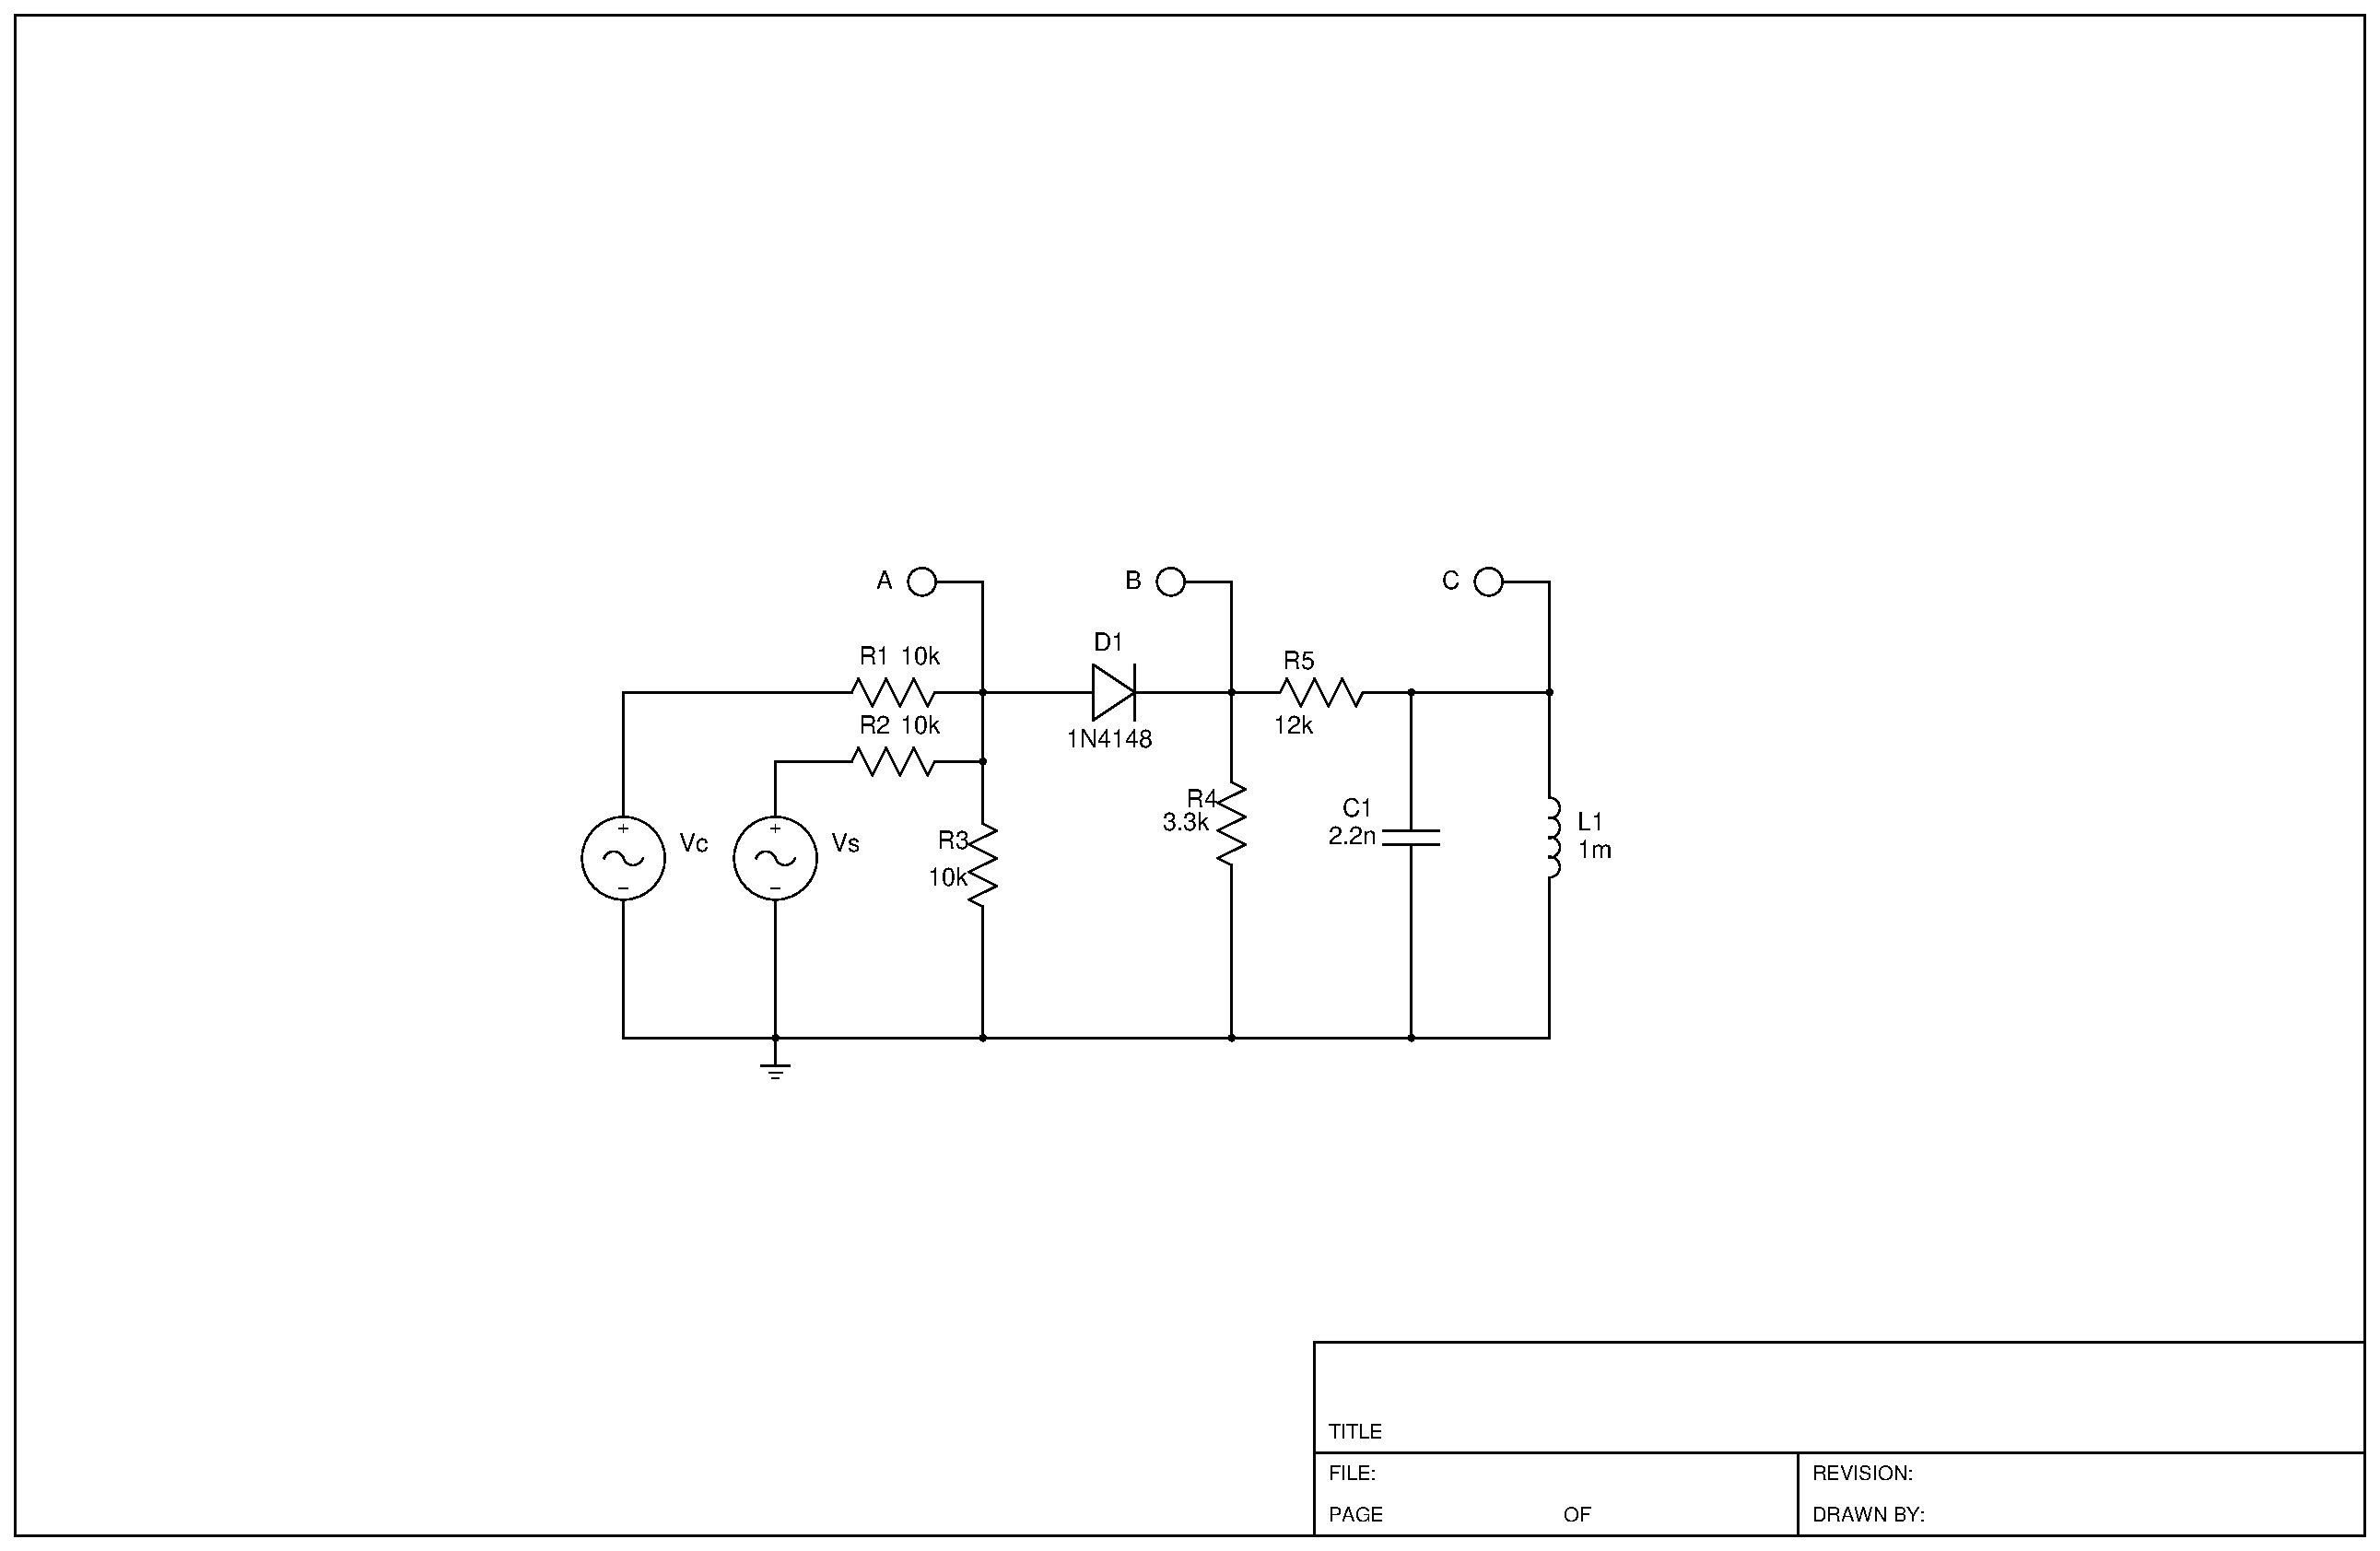
\includegraphics[scale=0.4,clip]{./imagens/AM_Modulator_Diode}
\end{center}
\caption{Modulador AM a diodo.}
\label{fig:demodulador_AM_diodo}
\end{figure}

Para sintonizar a portadora, calcula-se a frequência de ressonância do filtro LC da saída:

\begin{equation}
f_0 = \frac{1}{2 \pi \sqrt{LC}}
\end{equation}

Para os valores fornecidos ($C = 2,2 nF$ e $L = 1000 \mu F$) ter-se-á que essa frequência será de cerca de 107 KHz. 

Após sintonizados os sinais de portadora e da modulante, na saída (ponto C) constata-se a modulação do sinal. Neste contexto, o indutor e o capacitor agem no sentido de limitar a faixa de frequência do sinal modulado.

Disto se determinam:
\begin{itemize}
\item{\bf Frequências dos sinais portador e modulante:} 107 KHz e 1 KHz, respectivamente.
\item{\bf Índice de modulação:}
\item{\bf Forma de onda:}
\item{\bf Potência média do sinal:}


\end{itemize}
\subsection{Modulação por diodo}
Pergunta: \begin{flushright}
\textit{Explique como o diodo possibilita a modulação do sinal Eo (t) no circuito implemen-
tado na matriz de contatos e apresente o equacionamento que demonstra tal método
de modulação.}
\end{flushright}

Suponhamos o diodo como uma chave que permite apenas a passagem da região positiva da onda da portadora. Esse diodo pode ser considerado como um dispositivo não linear, expresso por $e_1(t) = a e_0(t) + b e^2_0(t)$. 

Ao diodo chega a soma dos sinais da portadora e da modulante: $e_0(t) = v_s + v_c$.

\subsection{Demodulação do sinal}

\chapter{Experimento 2: Modulação AM a transistor}

\begin{figure}[H]
\begin{center}
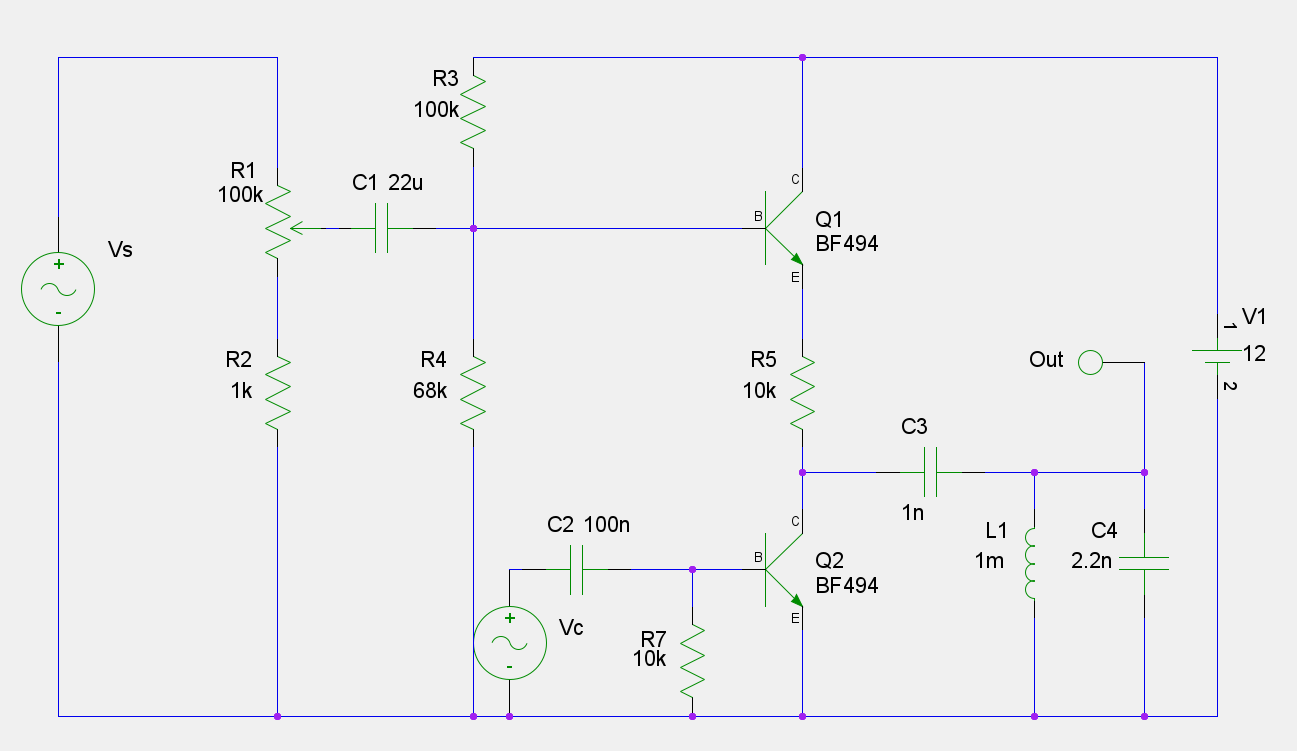
\includegraphics[scale=0.25,clip]{./imagens/AM_Modulator_Transistor.png}
\end{center}
\caption{Modulador AM a transistor.}
\label{fig:modulador_AM_transistor}
\end{figure}


O sinal modulado é gerado utilizando-se os transistores BF494 \cite{BF494}, de alta frequência (até 120 MHz, conforme sua \textit{datasheet}). O sinal de áudio oscila pelo transistor $Q_1$, e a portadora pelo transistor $Q_2$. Tal circuito se comporta como um multiplicador de sinais. A junção desses sinais é feita no capacitor $C_3$, que já remove qualquer nível DC que exista na saída dos transistores, e o filtro LC formado por $L_1$ e $C_4$ tratará de permitir apenas o nível de sinal relevante.

\chapter{Experimento 3: Transmissão e recepção de FM}
\section{Demodulação FM}
Ela também pode ser feita utilizando-se um circuito PLL (\textit{Phase-Locked Loop}), o qual foge do foco do presente trabalho.
\chapter{Experimento 4: Modulação por código de pulso (PCM)}
\section{Introdução}
PCM é uma técnica para a representação de sinais analógicos convertidos para formato digital, visando transmissão ou posterior processamento. Uma codificação em PCM transforma uma amostra quantizada em um número codificado. \cite{renatodatacom}

Fundamentalmente, a técnica consiste na quantização dos dados através de um conversor A/D. No lado do receptor existirá um conversor D/A que irá fazer o processo oposto.

\bibliographystyle{alpha}
\begin{thebibliography}{100}
\bibitem{renatodatacom}
 MACHADO, R. 
 \textbf{Notas de aula da disciplina de Comunicação de Dados.}
 Disponível em \url{http://www.ufsm.br/gpscom/professores/Renato\%20Machado/comunicacaodedados.html}. Acessado em 12/06/2012.
 
\bibitem{wolframeuler}
 \textbf{Euler Formula}. Disponível em \url{http://mathworld.wolfram.com/EulerFormula.html}. Acessado em 23/06/2012.

\bibitem{lamar}
LAMAR, V. M. \textbf{Modulação em Amplitude}. Disponível em \url{http://www.cic.unb.br/~lamar/te060/Apostila/Capitulo2.pdf}. Acesso em 23/06/2012.

 
\bibitem{BF494}
\textbf{BF494, BF495 NPN Medium-Frequency Transistors}. Disponível em \url{http://www.datasheetcatalog.org/datasheet/philips/BF494B.pdf}. Acesso em 23/06/2012.


\end{thebibliography}
\end{document}          
